\section{Research}

We aim to build a visual analytics system that can be used in understanding social behaviors and urban activities. This is done through two key steps, namely

\begin{itemize}
\item Extract events from taxi data
\item Analyze social media conversations corresponding to the events
\end{itemize}

Combining these two steps, we proposed a framework that can be used in interactively exploring different events around a city across time, using these observations to draw hypotheses and apply the findings in various fields.

\subsection{Analytical Frameworks}
In this section, we further detail the analytical frameworks that we used for the two key steps mentioned above.

\subsubsection{Taxi Data Analysis}
To extract events from the taxi data, we use Topological Data Analysis (TDA) to identify the maxima and minima events across the spatio-temporal data. Conneau et al. \cite{xlmroberta} used TDA to extract events from taxi data. Miranda et al. \cite{miranda2017Urban} also extracted urban pulses from scalar data of Flickr photo counts. First, we will aggregate the taxi data into a scalar function by applying a Gaussian kernel on it. Here, we use the total drop off in a particular latitude-longitude to create the aggregation so that we can explore other aggregations that might produce more meaningful results. For example, comparing the trends of total drop offs by date to the average deviation from weekday mean showed in (Fig.~\ref{fig:dailytrends}). It is clear that the latter might be able to identify more interesting events which might be produce better results for our use-case. However, this process will be explored further as our future work.

We then apply a lowerstar filter on top of the scalar image and compute the persistence of various events in the data. We filter out the events with the highest lifetime to identify the maxima events and map it back to a latitude-longitude. The same can be performed for a range of dates to identify all such events of interest from the spatio-temporal data. With this our first step is completed. This process is depicted visually in Fig.~\ref{fig:tda}. These experiments were carried out using the Ripser python TDA package \cite{ripser}.

\begin{figure}[ht]
 \centering % avoid the use of \begin{center}...\end{center} and use \centering instead (more compact)
 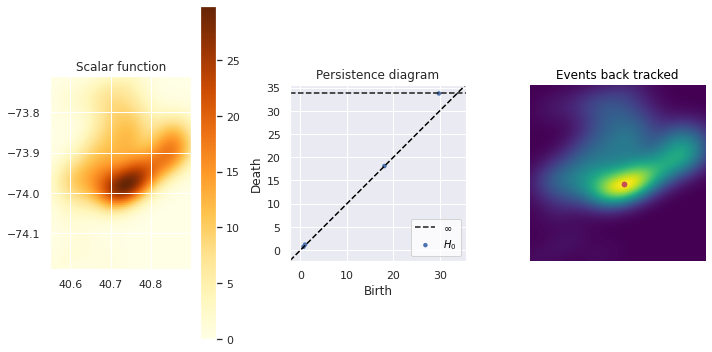
\includegraphics[scale=.25]{final/fig/TDA.png}
 \caption{Topological analysis of daily taxi trips}
 \label{fig:dailytrends}
\end{figure}


\subsubsection{Twitter Analysis}

Analyzing the twitter data entails two sub-tasks - 1. Topic modeling to understand what topics the conversations in specific areas are revolving around, 2. Sentiment analysis of these topics.

\textbf{Topic Modeling : }
We first explored the prevalent Latent Dirichlet Allocation algorithm, a probabilistic model that typically used for topic modeling. We used the Gensim \cite{gensim} python package for all experiments related to topic modeling. The general process of Topic modeling is the same as any natural language tasks and involves data cleaning (removing punctuation, stop words etc.), then lemmatization and finally feeding the documents (each instance of tweet here is referred to as a document) into a topic model. The LDA algorithm then iteratively trains on all these documents to model the representation of topics and their relation to the terms (i.e. words) present in the documents. Once trained, the model can be used to predict the topic present in a particular document as a probability distribution.

The joint probability in LDA is formulated as:

$${\delta = \prod_{d=1}^{D} p(\Theta_d|\alpha) 
\prod_{n=1}^{N} p(z_{d,n}|\Theta_d)p(w_{d,n}|\beta_{1:K},z_{d,n})}$$

$${p(\beta, \Theta, z | w) = \prod_{i=1}^{K} p(\beta_i | \eta) \delta
}$$

Where $\beta_k$ for a topic k is its word distribution, $\Theta$ is the topic proportions of a document, z is the topic assignment of a word, $\eta$ is the topic parameter and $\alpha$ is the proportions parameter.

We found that applying LDA had two key drawbacks. First, the topics and the key terms representing these topics were not known beforehand and remain static. The lack of dynamic change and addition of new key terms limits LDA's ability to model current events. Consequently, the coherence score of various iterations of the models were also poor (ranging between 30-50\%). Second, LDA is usually applied for documents of larger sizes, that produces more coherent topics. We also tried some workarounds by concatenating tweets from a day to produce a larger document, that did not improve the performance much. For these reasons, we moved on to explore an alternate methodology.

\begin{figure}[ht]
 \centering % avoid the use of \begin{center}...\end{center} and use \centering instead (more compact)
 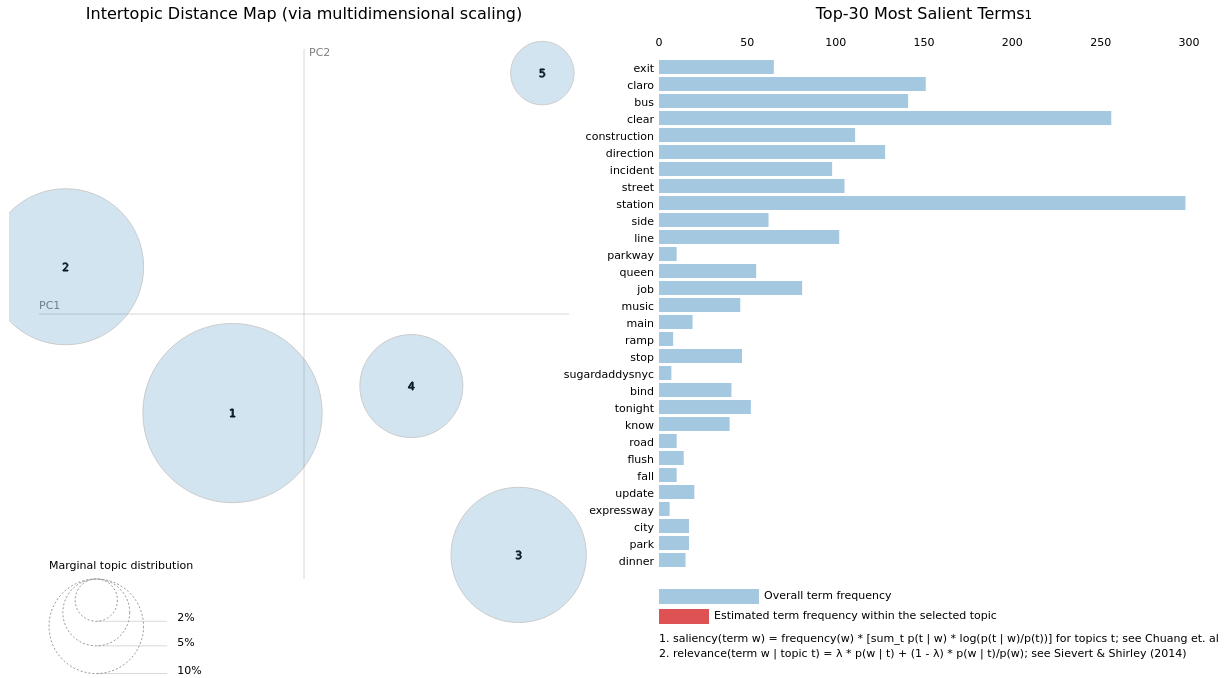
\includegraphics[scale=0.15]{final/fig/LDA.png}
 \caption{Topic Modeling results showing the created topics and their key terms to the right}
 \label{fig:tda}
\end{figure}

\textbf{Sentiment Analysis: }
In order to gain an understanding about the thoughts and associated feelings of users in our study, we required a tool to analyze the emotions behind posts made by each user. For this reason, we used data from the Twitter dataset and applied a discrete classification of sentiment into positive, negative and neutral in order to establish a suitable parameter to judge human feelings and behavior. 

In our first step, we cleaned and preprocessed the tweet using stemming, stop-word removal, and keyword extraction. Then, we applied the NLTK library`s sentiment classification on it to determine its respective scores for each sentiment. These scores would then be passed through a set threshold which helps us classify which sentiment a tweet belongs to.  Furthermore, besides classifying tweets, we also extracted general sentiment for each keyword for every hour, day and month respectively, thus allowing us to better analyse trends in sentiment change regrading any term over different duration. In our research, we emphasised on days with special events such as Halloween, Christmas, Thanksgiving and the New Year Eve.

While using NLTK provided us with a general sense of how users felt, we still felt the need for a more granular description of what the user felt to improve our analysis. In order to delve deeper and have more defined sentiments, we tried other approaches such as the Zero Shot Model which provided more depth and variations in the kinds of sentiment we could model. We will cover this in the next subsection.

\textbf{Zero Shot Model : }
In order to alleviate the drawbacks mentioned above we shifted from our initial task of Topic Modeling, to Topic Classification. As our analysis is mainly related to urban activity, we came up with some labels for topics such as ``Traffic/Construction'', ``Holiday/Celebration'', ``Politics'', ``Sports'', and other major seasonal events such as ``Halloween'', ``Thanksgiving'' and ``Christmas''.

We used a pre-trained language model that was trained on a multi-lingual dataset for a Natural Language Inference (NLI) task. NLI tasks have the setup of a premise and hypothesis and predicts whether the premise ``entails'', ``contradicts'', or is ``neutral'' to the hypothesis. We use the probability of ``entail''-ment as the probability of classification for the given labels. The underlying model is the XLM-RoBERTa language model\cite{xlmroberta} and we use the HuggingFace transformers pipeline to perform this inference.

One current drawback of this approach is that the inference takes a long time (~10 minutes for 10,000 tweets). We explored some parallel processing approaches to alleviate this with no success so far. We used this model for both Topic and Seniment classification (with labels such as - ``happy'', ``sad'', ``excited'' etc.)

\subsection{Implementation}

\subsubsection{System Architecture}
\begin{figure}[ht]
 \centering % avoid the use of \begin{center}...\end{center} and use \centering instead (more compact)
 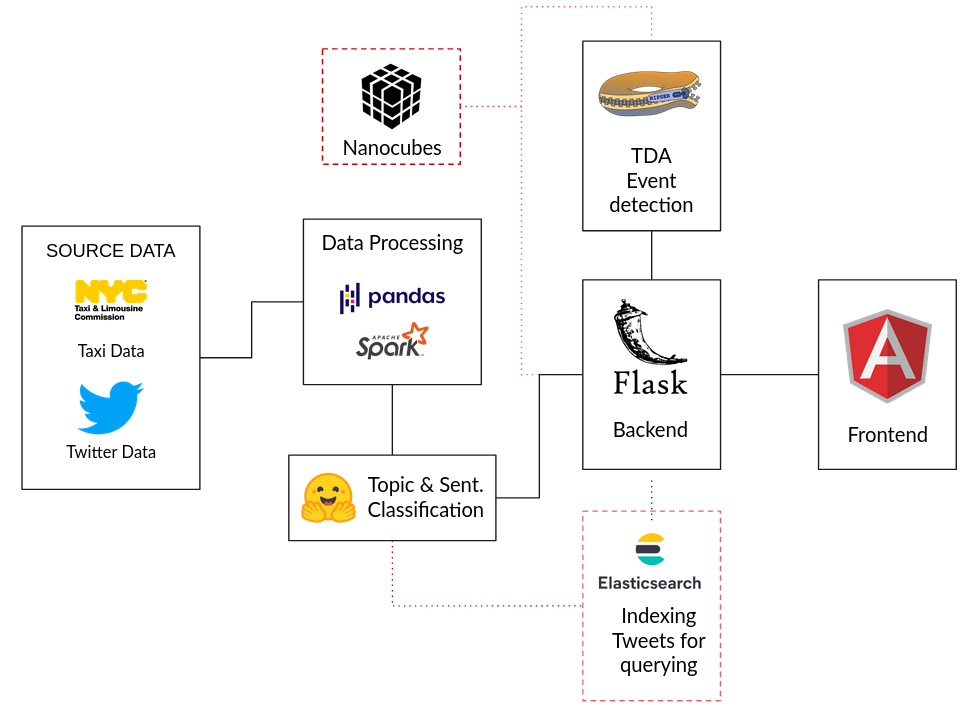
\includegraphics[width=\linewidth]{final/fig/system_arch.png}
 \caption{System architecture of the proposed visual analytics system}
 \label{fig:architecture}
\end{figure}


% \begin{figure*}[t]
% \centering
% \rule{\linewidth}{3cm}
% \caption{Wide single column figure in a twocolumn document.}
% \end{figure*}

We propose the following architecture for our visual analytics system  as depicted in (Fig.~\ref{fig:architecture})

There are three layers:
\begin{itemize}
    \item Source data:
        \begin{itemize}
            \item Consists of the three primary data sources - NYC Taxi trip data and Twitter data
            \item Data was be ingested from these sources through direct data pull, will be eventually automated to extract data for all available years
        \end{itemize}
        
    \item Data Management:
        \begin{itemize}
            \item In this layer, we performed the necessary cleaning and aggregation of taxi data at a daily level
            \item Pandas and Spark libraries were used to perform aggregation and to speed up the pre-processing steps such as mapping a tweet and taxi ride records to a specific taxi zones
            \item We also use the HuggingFace Zero-shot pipeline to infer topic and sentiment for all the tweets in this layer
            \item Additionally, we will perform TDA on the aggregated Taxi data to extract events of interest using the Ripser package
        \end{itemize}
    \item Visual System:
        \begin{itemize}
            \item The visual system is used to depict a visual representation of the extracted Taxi events and will allow for interactive exploration of selected events along with the topic and sentiment of the tweets corresponding to the selected event
            \item The system currently has an Angular front end and the Flask backend is a work in progress. Once functional, the Flask backed will serve the entire application and co-ordinate fetching information from the data management layer
        \end{itemize}
    \item Other Components:
        \begin{itemize}
            \item We also have two other components planned for the system that are yet to be explored
            \item We would use Nanocubes to serve aggregated Taxi data, to perform live event extraction on selected spatio-temporal constraints
            \item We would also use Elasticsearch to index and serve Tweets with their topics and sentiment to fetch results for a given constrains in a scalable manner
        \end{itemize}
\end{itemize}



\subsection{Task Analysis}
A description of the tasks are given below - 
\begin{itemize}
  \item Visualize big spatio-temporal data efficiently without any significant delay.
  \item What are the hotspots around the city throughout the different times of the year? What are the general trends and patterns in the taxi trips throughout the city?
  \item Identify any surge or drops in taxi pick-ups or drop-offs at certain locations in temporal space and explain the reason for such cases in terms of environmental change and social events
\end{itemize}
 
\subsection{Visual Interface}
\begin{figure}[ht]
 \centering % avoid the use of \begin{center}...\end{center} and use \centering instead (more compact)
 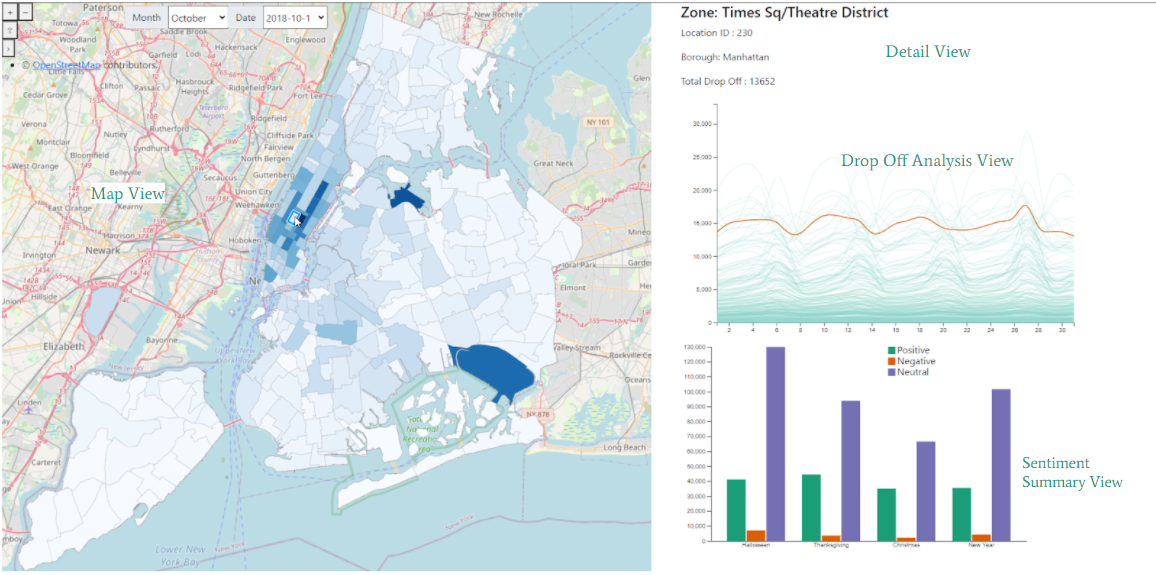
\includegraphics[width=\linewidth]{final/fig/interface.PNG}
 \caption{Visual interface of the proposed system}
 \label{fig:interface}
\end{figure}
We present a visual interface to to explore taxi and twitter data. The interface consists of four main views - Map view, Detail view, Drop Off Analysis View, Sentiment Summary view. 

\textbf{Map view} shows a heat map of New York City based on the taxi drop offs of NYC taxi zones for a selected date. User can select date and month from the dropdown menus. When user selects a zone from the map, the \textbf{detail view} shows relevant information such a zone name, location id, borough name and the drop off count. The \textbf{Drop Off Analysis View} shows the dropoff counts for a selected a month for all taxi zones. This view allows users to understand the change in drop offs over time. When user selects a zone from the map view, the selected zone is also highlighted in the dropoff analysis view. Finally, \textbf{Sentiment Summary View} shows the sentiments of the tweets based on topics such as Halloween, Thanksgiving, Christmas and so on.

